\documentclass[11pt, oneside]{article}   	% use "amsart" instead of "article" for AMSLaTeX format
\usepackage{geometry}                		% See geometry.pdf to learn the layout options. There are lots.
\geometry{letterpaper}                   		% ... or a4paper or a5paper or ... 
%\geometry{landscape}                		% Activate for for rotated page geometry
%\usepackage[parfill]{parskip}    		% Activate to begin paragraphs with an empty line rather than an indent
\usepackage{graphicx}				% Use pdf, png, jpg, or eps� with pdflatex; use eps in DVI mode
								% TeX will automatically convert eps --> pdf in pdflatex		
\usepackage{amssymb}
\usepackage{amsmath}
\usepackage{parskip}
\usepackage{color}
\usepackage{hyperref}

\title{Problems}
%\author{The Author}
%\section{}
%\subsection*{}
\date{}							% Activate to display a given date or no date

\graphicspath{{/Users/telliott_admin/Dropbox/Tex/png/}}
% \begin{center} 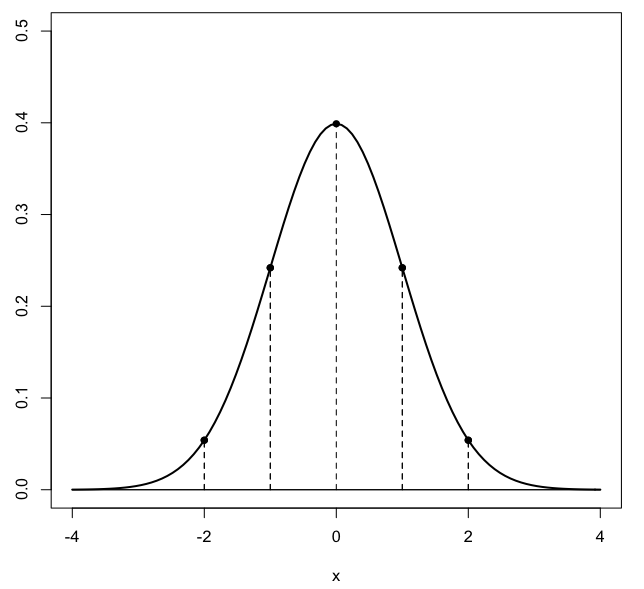
\includegraphics [scale=0.4] {gauss3.png} \end{center}
\begin{document}
\maketitle
\Large
\subsection*{example}
\[ \int e^x \cos x \ dx \]
Let
\[ u = e^x, \ \ \ du = e^x \ dx \]
\[ dv = \cos x  \ dx, \ \ \ v = \sin x \]
Then the integral is $uv - \int v \ du$ or
\[ = e^x \sin x - \int e^x \sin x \ dx \]
which looks like no help, but keep going.  Lather, rinse, repeat:
\[ u = e^x, \ \ \ du = e^x \ dx \]
\[ dv = - \sin x \ dx, \ \ \ v = \cos x \]
Then the second integral is
\[ - \int e^x \sin x \ dx = e^x \cos x - \int e^x \cos x \ dx \]
Putting the answers together:
\[ \int e^x \cos x \ dx = e^x \sin x + e^x \cos x - \int e^x \cos x \ dx \]
so
\[ 2 \int e^x \cos x \ dx = e^x \sin x + e^x \cos x \]
\[ \int e^x \cos x \ dx = \frac{1}{2} \ e^x \ [ \ \sin x + \cos x \ ] \]
Check by differentiating.  Leave the factor of $1/2$ aside for the moment:
\[ \frac{d}{dx} \ e^x \ [ \ \sin x + \cos x \ ] \ = e^x \ [ \ \sin x + \cos x \ ] + e^x \ [  \ \cos x - \sin x \ ] \]
The $\sin x$ terms cancel, giving $2$ terms of $\cos x$ but we have the factor of $1/2$ so that finally gives:
\[ \frac{d}{dx} \ e^x \ [ \ \sin x + \cos x \ ] \ = e^x \cos x  \]


\end{document}  